\subsection{Euler-Maclaurin公式}
  \paragraph{绪论}
   此节内容的主要是对 Apostol, T. M. (1 May 1999).
   "An Elementary View of Euler's Summation Formula"
   的翻译和整理.

  \subsubsection{广义Euler常数}
    \paragraph{绪论}
      本章节仅考虑在$[1,\infty)$上满足$\f>0$,且严格单调递减的函数.

    \begin{defi}[$d_n$]
      定义$d_n$为用积分近似离散求和的误差,即
      \begin{equation}
        \label{equ: d_n}
        d_n = \sum_{k=1}^{n-1}\f(k) - \int_1^n\f(x)\rd x
      \end{equation}
    \end{defi}
    \remark
      注意,$d_n$的定义中,$k$仅遍历$[1, n-1]$,而不包含$n$.
      \begin{figure}[htbp]
        \centering
        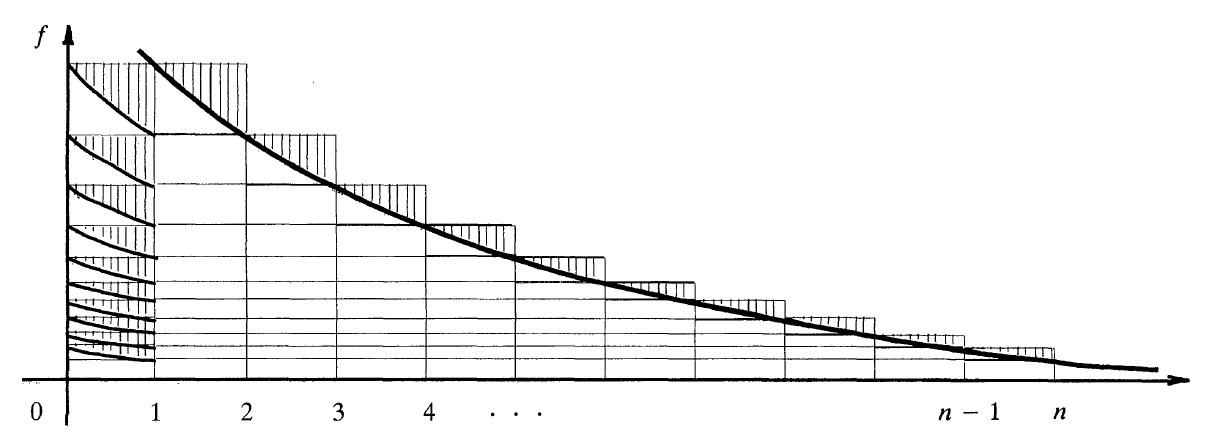
\includegraphics[width=15cm]{../image/d_n.png}
        \caption{$d_n$的几何解释}
        \label{fig: d_n的几何解释}
      \end{figure}
      \figref{fig: d_n的几何解释}为$d_n$的几何解释,其中
      在曲线上方的阴影部分即为$d_n$,可以将它们统一移动到图像的最左侧.

    \begin{defi}[广义Euler常数]
      已知$0<d_n<d_{n+1}<\f(1)$,所以可以定义关于$\f$的广义Euler常数
      $C(\f)$为
      \[
        C(\f) = \lim_{n\to\infty}d(n)
      \]
    \end{defi}

    \begin{pos}[余项估计]
      $0 < C(\f) - d_n < \f(n)$.
    \end{pos}

    \begin{thm}
      设$\f$在$[1,\infty)$上为正且严格单调递减,则存在一列
      $\{E_{\f}(n)\}$,满足$0<E_{\f}(n) < \f(n)$,成立
      \begin{equation}
        \sum_{k=1}^n\f(k) = \int_1^n\f\rd x + C(\f) + E_{\f}(n),
        \quad n = 2,3,\dots.
      \end{equation}
    \end{thm}
    \remark
      只需令$\lhs = \sum_{k=1}^{n-1}\f(k) + \f(n)$,在根据$d_n$
      的定义即可证明. 这一定理意味着求和与积分之间的误差仅仅为一个与
      $\f$有关的常数以及一个比$\f(n)$还要小的正数. 从而如果$\f(n)\to 0$,
      则$E_{\f}(n)\to 0$,此时成立
      \begin{equation}
        C(\f) = \lim_{n\to\infty}\left(
          \sum_{k=1}^n \f(k) - \int_1^n\f(x)\rd x
        \right).
      \end{equation}

    \begin{defi}[经典Euler常数]
      取$\f(x) = 1/x$,它满足$\lim_{x\to\infty}\f(x) = 0$,则有
      \[
        \gamma = C(\frac{1}{x}) = \lim_{n\to\infty}\left(
          \sum_{k=1}^n\frac{1}{k} - \ln n
        \right).
      \]
    \end{defi}

  \subsubsection{Euler求和公式}
    \paragraph{绪论}
      在此章节不再限制$\f$需要为正且单调减,在目前仅要求$\f\in\ms{R}[1, n]$
      (在之后会添加诸如连续可导等条件). 在此基础上重新定义$d_n$(与上一节保持一致)
      并推导出类似于上一节中的结论.

    \begin{defi}[$d_n$]
      定义$d_n$为
      \begin{equation}
        d_n = \sum_{k=1}^{n-1}I(k) =
        \sum_{k=1}^{n-1} \int_{k}^{k+1}\{ \f(k) - \f(x) \}\rd x.
      \end{equation}
    \end{defi}
    \remark
      可以发现这一定义和上一节中的定义,在$\f>0$且单调减的情况下是一致的.
      实际上这一定义只是将每一点处的差值积分起来而已.

    \begin{pos}
      对于任意常数$c$,由于成立$\rd x= \rd(x+c)$,所以可以取$c=-(k+1)$,并分部
      积分,则有
      \[
        I(k) = \int_{k}^{k+1} (x-[x]-1)\f\hp(x)\rd x.
      \]
      从而
      \[
        d_n = \int_1^n(x-[x])\f\hp(x)\rd x + \f(1) - \f(n).
      \]
    \end{pos}

    \begin{thm}[一次导数形式的Euler求和公式]
      对于任意$\f\in\ms{C}^1[1,n]$,成立
      \begin{equation}
        \label{equ: 一次导数Euler求和公式}
        \sum_{k=1}^n\f(k) = \int_1^n\f(x)\rd x +
        \int_1^n(x-[x])\f\hp(x)\rd x + \f(1).
      \end{equation}
    \end{thm}
    \remark
      对于误差项中的$\f\hp$,如果它不变号,即$\f$单调的情况下,
      可以考虑让它乘一个变号的因数,从而使得误差更小. 例如,可以
      用$x-[x]-\frac{1}{2}$来代替$x-[x]$. 则有了如下推论.

    \begin{cor}
      \label{cor: 一次Euler求和公式}
      对于任意$\f\in\ms{C}^1[1,n]$,定义一次Bernoulli函数为
      \[
        P_1(x) =
        \begin{cases}
          x - [x] - \frac{1}{2},\quad& x \notin \mbf{N} \\
          0, & x\in\mbf{N}.
        \end{cases}
      \]
      则可以重写\equref{equ: 一次导数Euler求和公式}为
      \begin{equation}
        \sum_{k=1}^n\f(k) = \int_1^n\f(x)\rd x +
        \int_1^nP_1(x)\f\hp(x)\rd x + \frac{1}{2}(\f(n) + \f(1)).
      \end{equation}
      若假设$\int_1^{\infty}P_1\f\rd x$存在,那么上式可以继续写为
      \[
        \begin{split}
        \sum_{k=1}^n\f(k) &= \int_1^n\f(x)\rd x + C(\f) + E_{\f}(n) \\
        C(\f) &= \frac{1}{2}\f(1) + \int_1^{\infty}P_1\f\hp\rd x\\
        E_{\f}(n) &= \frac{1}{2}\f(n) - \int_n^{\infty}P_1\f\hp\rd x
      \end{split}\]
    \end{cor}
    \remark
      注意,在此处$C(\f)$和$E_{\f}(n)$的定义和之前依然是一致的. 并且只需要
      $\f(x)$在$[1, \infty)$上反常绝对可积,就可以保证
      $\int_1^\infty P_1\f\rd x$的存在性.\footnote{我暂时并没有明白,是
      什么条件保证了$\f(n)\to 0$,从而$C(\f) = \lim_{n\to\infty}d_n$存在.}

    \begin{cor}[Euler常数]
      将$\f(x) = 1/x$,代入\corref{cor: 一次Euler求和公式},得
      经典Euler常数$\gamma$为
      \[
        \gamma = \frac{1}{2} = \int_1^\infty \frac{P_1(x)}{x}\rd x.
      \]
    \end{cor}

  \subsubsection{余项分析}
    \paragraph{绪论}
      这一章节通过对
      \begin{equation}
        \label{equ: Euler求和公式余项1}
        \int_n^{n+1}P_1(x)\f(x)\rd x
      \end{equation}
      分部积分来进一步分析余项,并为此引入了更高次的Bernoulli函数.

    \begin{defi}[二次Bernoulli函数]
      定义二次Bernoulli函数$P_2(x)$为
      \[
        P_2(x) = 2\int_0^xP_1(t)\rd t + \frac{1}{6}.
      \]
    \end{defi}
    \remark
      如此定义二次Bernoulli函数的动机来自于对
      \equref{equ: Euler求和公式余项1}的进一步分部积分. 这样就需要有
      \[
        P_2(x) = 2\int_0^xP_1(t)\rd t + c
      \]
      之所以要有系数$2$是为了之后公式的简洁. 由于$P_1(x)$有周期性,从而
      \[
        P_2(x+1) - P_2(x) = 2\int_x^{x+1}P_1(t)\rd t = 0,
      \]
      即$P_2(x)$也有周期性. 为了让按照同样方式定义的$P_3$也具有周期性,
      所以希望有
      \[
        \int_0^1P_2(x)\rd x= 0 \,\Rightarrow\, c = \frac{1}{6}.
        \quad\blacksquare
      \]

    \begin{thm}[二次导数形式的Euler求和公式]
      设$\f\in\ms{C}^2[1, n]$,成立
      \[
        \sum_{k=1}^n\f(k) = \int_1^n\f\rd x
        - \frac{1}{2}\int_1^nP_2\f^{\pr\pr}\rd x
        + \frac{1}{2}P_2(0)(\f\hp(n)-\f\hp(1))
        + \frac{1}{2}(\f(n) + \f(1)).
      \]
      并且,如果$\f^{\pr\pr}$在$[1, \infty)$上反常绝对可积,则有
      \[\begin{split}
        \sum_{k=1}^n\f(k) &= \int_1^n\f\rd x + C(\f) + E_{\f}(n) \\
        C(\f) &= \frac{1}{2}\f(1) - \frac{1}{2}P_2(0)\f\hp(1)
        - \frac{1}{2}\int_1^\infty P_2\f^{\pr\pr}\rd x \\
        E_{\f}(n) = \frac{1}{2}\f(n) + \frac{1}{2}P_2(0)\f\hp(n) +
        \frac{1}{2}\int_n^\infty P_2\f^{\pr\pr}\rd x.
      \end{split}\]
    \end{thm}

  \subsubsection{Bernoulli数和Euler求和公式的一般形式}
    \begin{defi}
      定义\tbf{Bernoulli周期函数}为
      \begin{equation}
          P_k(x) = k\int_0^x P_{k-1}(t)\rd t + B_k,\quad k\ge 2
      \end{equation}
      其中$B_k$称为\tbf{Bernoulli数},它使得下式成立
      \[
        \int_0^1P_k(x)\rd x = 0.
      \]
      显然$P_k(x)$在$k\ge 2$的时候在$[0, 1]$上是$k$次多项式,称
      它为\tbf{Bernoulli多项式}.
    \end{defi}

    \begin{thm}[等价定义]
      Bernoulli数和Bernoulli多项式的另一种常见定义为,
      \[\begin{split}
        & B_0 = 1,\quad \sum_{k=0}^{m+1} {{m+1}\choose{k}} B_k = 0 \\
        & B_n(x) = \sum_{k=0}^n{{n}\choose{k}}B_{n-k}x^k.
      \end{split}\]
    \end{thm}
    \remark
      对于大于$1$的奇数$k$,$B_k=0$,且有
      \[
        |B_{2k}(x)| \le |B_{2k}|,\quad
        |B_{2k+1}(x)| \le (2k+1)|B_{2k}|.
      \]

    \begin{thm}[Euler求和公式的一般形式]
      设$\f\in\ms{C}^{2m+1}[1, n]$,成立
      \[\begin{split}
        \sum_{k=1}^n\f(k) = & \int_1^n\f\rd x +
        \frac{1}{(2m+1)!}\int_1^n P_{2m+1}(x)\f^{(2m+1)}(x)\rd x\\
        & + \sum_{r=1}^m \frac{B_{2r}}{(2r)!}(\f^{(2r-1)}(n)-\f^{(2r-1)}(1))
        + \frac{1}{2}(\f(1) + \f(n)).
      \end{split}\]
      且若$\f^{(2m+1)}$在$[1, \infty)$上反常绝对可积,则成立
      \[\begin{split}
      \sum_{k=1}^n\f(k) &= \int_1^n\f\rd x + C(\f) + E_{\f}(n) \\
      C(\f) &= \frac{1}{2}\f(1) - \sum_{r=1}^m\frac{B_{2r}}{(2r)!}\f^{(2r-1)}(1)
      + \frac{1}{(2m+1)!}\int_1^{\infty}P_{2m+1}\f^{(2m+1)}\rd x \\
      E_{\f}(n) &= \frac{1}{2}\f(n) + \sum_{r=1}^m\frac{B_{2r}}{(2r)!}\f^{(2r-1)}(n)
      - \frac{1}{(2m+1)!}\int_n^{\infty}P_{2m+1}\f^{(2m+1)}\rd x
      \end{split}\]
    \end{thm}
